\chapter{Literature Review} % Main chapter title

\label{Chapter3} % For referencing this chapter elsewhere, use \ref{Chapter2}

\lhead{Chapter 3. \emph{Literature Review}}

%----------------------------------------------------------------------------------------
%	SECTION 3.1 - Mixed Precision
%----------------------------------------------------------------------------------------

\section{Mixed Precision}

The first section explained in details the different existing number representations. With a particular emphasis on the representation of floating-point number, it has shown what the underlying issues of such representations are. The question now is how can we use to our advantage the different types along with their strengths and weaknesses?

%-----------------------------------
%	SUBSECTION 3.1.1 - Motivations
%-----------------------------------
\subsection{Motivations}

The term \guille{mixed precision} comes from the idea of using different precisions (type representations) to increase the performance of a computation that would otherwise only use the highest available (or user-defined) precision. The previous section showed us that each number representation has its pros and cons. Using lower precision types and representations will allow the total computation to decrease the usage of several hardware resources (memory, bandwidth, energy consumption) \cite{Horowitz2014,Nips2015}.

However, if lower-precision is acceptable, using mixed-precision can increase the capacity of smaller systems and subsystems as it will increase the overall performance and resources usage. This goal is targeted when you are aiming for the most performant processor, being given a size and type of usage. Moreover, this can be used when you know exactly the tasks your system will perform as well as their needed size. Yates \cite{Yates2007} presents several rules allowing  to determine the required size of any operation performed in fixed-point arithmetic. This arithmetic allows to tailor the type size to one's needs. Reconfigurable hardware can take advantage of this as well by using the exact required size for an operation. Such architecture will be looked upon in the next sections.

Scientific computations often require the highest available precision and the reduced precision induced by the lower-precision components is unacceptable. In order to still take advantage of the several gains lower-precision provides, a compromise has to be found about how and when to use lower-precision. Ideas on the usage have been looked upon since the 1950's and the first methods to correctly implement them in the early 1960's.

In any case, the developer has to know and keep in mind:
\begin{itemize}
  \item Required end precision
  \item Acceptable error rate
  \item Actual operations performed by the system
\end{itemize}

Mixed precision methods consist of doing a large part of the computation in low-precision components and only a small part in high-precision. As presented in the survey paper \cite{Goddeke2007} using different formats in the same algorithm can have several beneficial properties such as:
\begin{itemize}
  \item Accuracy: Same accuracy when up to 99\% of the operations is performed in the low format
  \item Computation: Low precision operations require less transistors and can translate in more paralellism
  \item Memory: Reduction in size in memory influences the efficiency and bandwidth requirements positively
\end{itemize}

%-----------------------------------
%	SUBSECTION 3.1.2 - Methods and Implementations
%-----------------------------------

\subsection{Methods and Implementations}
Several methods to actually implement a mixed precision algorithm have been developed starting 60 years ago. If the methods are different in practice, the theory behind them is the same as they aim to delegate most of the work to low-precision components while only using high-precision to recover the desired accuracy for the computation.

%-----------------------------------
%	SUBSUBSECTION 3.1.2.1 - Iterative Refinement
%-----------------------------------

\subsubsection{Iterative Refinement}

Since the early 1960's, literature has studied the effects and ways to implement mixed precision. The first reported works to implement such methods are James H. Wilkinson \cite{Wilkinson1994} and Cleve Moler \cite{Moler1967}. The method presented by both is named \guille{iterative refinement} and uses a combination of accumulative inner products along with a linear solver. This solution is directed towards the resolution of a system in the form of $Ax=b$ for a quadratic $N*N$ matrix $A$. The main idea is to use a residual between the wanted result and the result obtained by the last iteration. This residual is computed using high precision and accumulated using high-precision as well while the resolution of the equation is done in low-precision.

% Iterative Refinement Example
\begin{figure}[htbp]
	\centering
\begin{tabular}{ll}
	$x^{(0)}=0$ &\\
	$d^{(s)}=b-Ax^{(s)}$ & Compute residual in \emph{high} precision\\
	$Ac^{(s)}=d^{(s)}$ & Solve equation system in \emph{low} precision\\
	$x^{(s+1)}=x^{(s)}+c^{(s)}$ & Accumulate solution in \emph{high} precision\\
\end{tabular}
	\caption[Iterative Refinement]{Iterative Refinement Method \cite{Goddeke2007}}
	\label{fig:IterativeRef}
\end{figure}

This method has later been reused and extended. Baboulin et al. \cite{Baboulin2009} combine single- and double-precision floating-point numbers to enhance the performance of \guille{dense and sparse linear algebra algorithms}. Strzodka et al. \cite{Strzodka2006} present an enhanced algorithm to resolve a partial differential equation (Poisson problem) to present the effects of a mixed-precision approach. Sun et al. \cite{Sun2008} reproduce a linear solver in mixed-precision but adds an error analysis. The last two articles implement the result of their research on a reprogrammable architecture. Several applications profit directly from these papers and their implementations of mixed-precision algorithms as seen in later sections.

%-----------------------------------
%	SUBSUBSECTION 3.1.2.2 - Iterative Refinement
%-----------------------------------

\subsubsection{Analysis and Rewriting}

When creating a new application or system, any developer tends to use the highest available (or one of the highest) to represent the numbers he will need. However, the space and operations performed on higher-precision types are, as shown earlier, not the most performant. A simple, yet effective way to choose the correct type is to analyse the code and rewrite types that can be represented by lower precision ones. This idea has been implemented in the code analysis tool Precimonious \cite{Rubio2013} for floating-point representations. This analysis tool can go over the code and determines parts of it where lower precision can apply.

The mixed-precision approach can apply from a different perspective when using a fixed-precision representation. Darulova et al. \cite{Darulova2013} show that several polynomial expressions over the reals are cast over fixed-point arithmetic without being optimised, leading approximations of the real values. The tool they present allows to determine the best fixed-point implementation of a real number thanks to genetic programming. Then, as the order of operations is impactful when dealing with fixed-point arithmetic (distributivity and associativity are not respected), the tool reorder the operations to optimise the error and accuracy.

Those two tools have been brought together in \cite{Darulova2018} under the \guille{first fully automated and sound technique and tool for optimising the performance of floating-point and fixed-point kernels}. This tool combines rewriting and mixed-precision tuning where rewriting goes over several evaluation orders and picks the one that minimises the round-off error without runtime costs. In the meantime, mixed-precision tuning assigns the correct finite-precision variables and operations. The overall tool provides finer-grain control over the program and better performance than each of the method taken alone.
% TUNING EXAMPLE
\begin{figure}[htbp]
\centering
\begin{minipage}{.48\textwidth}
\begin{lstlisting}[style=CInputStyle]
long double fun( long double x ) {
  int k, n = 5;
  long double t1;
  long double d1 = 1.0L;
  t1 = x;
  for( k = 1; k <= n; k++ ) {
    d1 = 2.0 * d1;
    t1 = t1 + sin (d1 * x) / d1;
  }
  return t1;
}
int main( int argc, char **argv) {
  int i, n = 1000000;
  long double h, t1, t2, dppi;
  long double s1;
  t1 = -1.0;
  dppi = acos(t1);
  s1 = 0.0;
  t1 = 0.0;
  h = dppi / n;
  for( i = 1; i <= n; i++ ) {
    t2 = fun (i * h);
    s1 = s1 + sqrt (h*h + (t2 - t1)*(t2 - t1));
    t1 = t2;
  }
  // final answer is stored in variable s1
  return 0;
}
\end{lstlisting}
\end{minipage}
\hfill
\begin{minipage}{.48\textwidth}
\begin{lstlisting}[style=CInputStyle]
double fun( double x ) {
  int k, n = 5;
  double t1;
  float d1 = 1.0f;
  t1 = x;
  for( k = 1; k <= n; k++ ) {
    d1 = 2.0 * d1;
    t1 = t1 + sin (d1 * x) / d1;
  }
return t1;
}
int main( int argc, char **argv) {
  int i, n = 1000000;
  double h, t1, t2, dppi;
  long double s1;
  t1 = -1.0;
  dppi = acos(t1);
   s1 = 0.0;
  t1 = 0.0;
  h = dppi / n;
  for( i = 1; i <= n; i++ ) {
    t2 = fun (i * h);
    s1 = s1 + sqrt (h*h + (t2 - t1)*(t2 - t1));
    t1 = t2;
  }
  // final answer is stored in variable s1
  return 0;
}
\end{lstlisting}
\end{minipage}
\caption[Tuning]{Tuning Example \cite{Rubio2013}}
	\label{fig:Tuning}
\end{figure}

%---------------------------------------------------------
%	SECTION 3.2 - Quantised Networks and Quantisation Methods
%---------------------------------------------------------
\section{Quantised Networks}

Machine learning can also benefit from mixed-precision since it is heavily relying on matrix operations. In the recent years, machine learning, and especially deep learning, are benefitting from the research in mixed-precision. There is a clear emphasis on either speeding up the training process or making the inference quicker. In this section we will be looking at neural networks using reduced precision. These types of networks are called \emph{Quantised Neural Networks} or \emph{QNN}.

%------------------------------------------------
%	SUBSECTION 3.2.1 - Introducing Mixed Precision
%------------------------------------------------

\subsection{Introducing Mixed Precision}

Training a neural network is the longest process, among mandatory ones, to make the most out of the architecture. However, mixed-precision mindset offers ways to accelerate the training of the network by decreasing the precision of some operations. The ImageNet Project \cite{ImageNet2009} is a large database designed to be used in visual object recognition softwares.  While accuracy is the main factor to determine the winner, deep learning real-world issues often have to take in account the network's training phase.

The benchmarks in this field use several metrics in order to quantify and qualify the networks and their implementations.
\begin{itemize}
	\item \textbf{Parameters' Size}: The size or precision of parameters of the network: weights and activation functions.
	\item \textbf{Network Layout}: The configuration of the neural networks with the number, size and type of layers.
	\item \textbf{Accuracy}: The ratio of the number of correct precisions out of the total number of predictions. \emph{The higher the better}.
	\item \textbf{Training Time}: The cost of operations in a given representation. \emph{The lower the better}.
\end{itemize}

Many researchers have been looking into the issue with mixed-precision in mind. As shown by Bacchus et al. \cite{Bacchus2020}, there is a fundamental underlying trade-off between accuracy, network training time and hardware efficiency. Research looked upon ways to reduce the size taken by weights and the activation function and the impact of a reduction in the size of those:

Micikevicius et al. \cite{Micikevicius2017} store weights, activations and gradients in IEEE half-precision nearly halving the memory requirements and speeding up the arithmetic. The authors propose three techniques to maintain the accuracy of the model. They maintain a single-precision copy of weights to accumulate the gradients, propose a loss-scaling to preserve low-magnitude gradients and use half-precision arithmetic that writes to single-precision arithmetic before writing the half-precision values to memory.

Colangelo et al. \cite{Colangelo2018} present a CNN mapping to a reconfigurable architecture in order to use sub 8-bit activation and weights. In order to use binary- or ternary-weighted neural networks, they cap their sizes to respectively 1 and 2-bits. Using this type of limited numeric precision can only be fully optimised with FPGAs and the authors show that they manage to get an optimisation of \guille{the bandwidth, memory, power and computation savings}.

Jia et al. \cite{Jia2018} present a novel mixed-precision training method along with an optimised all-reduce algorithm. Any neural network will have to use a version of an all-reduce algorithm, consisting of the sum of all the previous elements broadcasted to all the next elements. Using an optimised version of the algorithm will increase the performance of each layer separately and the whole system in the end.

Zhao et al. \cite{Zhao2016} propose F-CNN, a framework to train CNNs on FPGAs. Their design makes available highly customisable modules that will be optimised to maximise performance under the constraints of bandwidth and hardware resources. The authors state that the introduction of mixed-precision will be the next step of optimisation of their design. Moreover, the use of they prove their design is more performant than CPUs and less expensive in terms of energy than GPUs.

Jahanshahi et al. \cite{Jahanshahi2019} propose a CNN accelerator tool. It generates the hardware description for a CNN to be programmed on a target FPGA. The software uses an API the developer can use to enter the available resources. The software will then generate the hardware description and run a simulation to adjust the precision and minimise the classification error. The whole system is shown to be more performant on a half-precision fixed-point representation rather than using single-precision floating-point data: 3\% accuracy loss in exchange for 15.75x speedup.

Kurth et al. \cite{Kurth2018} presents a direct application of mixed-precision training on GPUs to help climate analysis. The authors expand open-source tools such as Tensorflow and Horovod in order to present their work. They managed to optimise the network's training to increase the overall efficiency and performance. The predictions the network is able to make are shown to be of an unmet precision and will help characterise the impact of several physical events (flooding, monetary loss, etc.).

%-------------------------------------
%	SUBSECTION 3.2.2 - Quantisation Methods
%-------------------------------------

\subsection{Quantisation Methods}


%-----------------------------------
%	SECTION 3.3 - CNNs on FPGAs
%-----------------------------------

\section{CNNs on FPGAs}

Due to their heavy parallel affinity, CNNs can benefit from both GPUs \cite{Micikevicius2017, Jia2018, Kurth2018} and FPGAs \cite{Park2016, Liang2017, Colangelo2018, Jahanshahi2019, Bacchus2020} heavy parallelisation capabilities.
However, CNNs as stated in \cite{Jahanshahi2019}, "CNN-based methods are computational-intensive and resource-consuming, and thus are hard to be integrated into embedded systems such as smartphones, smart glasses and robots". FPGAs can counterbalance this issue by providing a tailored hardware representation of the CNN and making the most our of limited precision datatypes.

\cite{Zhao2016, Colangelo2018, Jahanshahi2019} presented frameworks for CNNs automatic or semi-automatic hardware implementations on FPGAs. Abdelouahab et al. \cite{Abdelouahab2018} present the issues FPGAs face and resolve in a survey paper. While this paper cites over a hundred sources, the following sections focuses on the main ideas it highlights.

%--------------------------------------------
%	SUBSECTION 3.3.1 - Parallelisation Vectors
%--------------------------------------------

\subsection{Parallelisation Vectors}

Low-energy embedded systems can take advantage of the affinity of CNNs with parallelisation. This extensive concurrency can be used when parallelising from either \emph{Batch Parallelism} or \emph{Inter-Layer Parallelism}.

Batch size is an important parameter when looking at networks, it corresponds to \guille{a hyper-parameter that defines the number of samples to work through before updating the internal model parameters (weights)} \cite{MLMastery2019}. As stated in \cite{MLMastery2019}, the difference between a \emph{batch} and an \emph{epoch} is that an epoch consists of a full run through the training set while several batches can fit into an epoch. The batch size can divide the training in several types depending on the batch size:

\begin{itemize}
	\item \emph{Batch Gradient Descent}: Batch size = Size of the training set
	\item \emph{Stochastic Gradient Descent}: Batch size = 1
	\item \emph{Mini-batch Gradient Descent}: 1 $<$ Batch size $<$ Size of the training set
\end{itemize}

A CNN can simultaneously run the filters of the network on the instances of the same batch and obtain a significant acceleration when using batch processing. On the other hand, the structure of the network can be described as \guille{feed-forward}, meaning the output of layer $n$ is directly fed into layer $n+1$. A pipelined implementation can trigger the layer $n+1$ before the end of layer $n$ on selected instances.

The layers CONV are source of concurrency that can be exploited through the separation of the different planes the CONV layer uses (inter-FM), or the separation of the outputs of the layer (intra-FM). Moreover, the 3D-convolution can be expressed as a sum of 2D-convolutions that can be executed in parallel (inter-convolution) and the 2D-convolutions themselves can be pipelined concurrently (intra-convolution).

%---------------------------------------------------------
%	SUBSECTION 3.3.2 - Training and Inference Optimisations
%---------------------------------------------------------

\subsection{Training and Inference Optimisations}

As said earlier, the \emph{Inference} step is a critical spot of CNN implementations as it is required each time a new instance is presented to the system whereas the \emph{Training} step can be done once and for all. Increasing the performance of this step is crucial and can be done in several ways. First, the memory bandwidth is the bottleneck of several FPGA implementations. High number of memory reads or high number of weights stored result in a loss of performance. A caching strategy is often a nice answer to this kind of issues.

Next, the literature presents several \emph{Inference Optimisations} strategies that will help the CNN perform best on an FPGA. Exporting a CNN to an FPGA consists in finding the most efficient way to map the CNN on the hardware architecture of the FPGA. The main strategies are listed beneath and presented in \emph{Figure} \ref{fig:InferenceOpt}.

% INFERENCE OPTIMISATIONS
\begin{figure}[htbp]
	\centering
		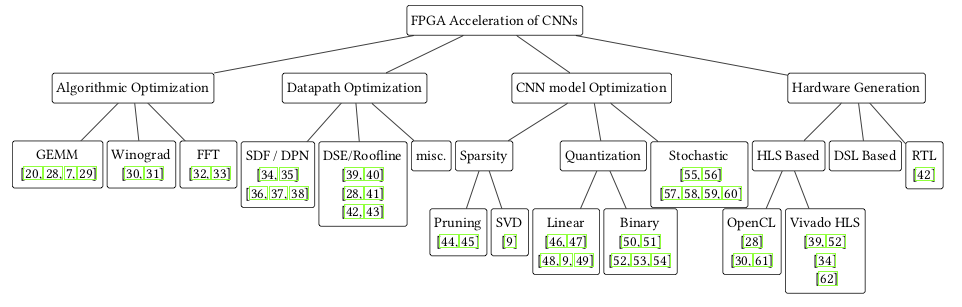
\includegraphics[width=\textwidth]{Figures/InferenceOpt.png}
	\caption[Inference Optimisations]{Methods to accelerate an FPGA implementation \cite{Abdelouahab2018}}
	\label{fig:InferenceOpt}
\end{figure}

The main strategies are:
\begin{itemize}
	\item Algorithmic optimisations: GEMM transformation, Winograd transform, Fast Fourier Transform .
	\item Data-path optimisations: Systolic arrays, SIMD and loop optimisations, Data-flow MoC.
	\item Approximate computations: Fixed-point, Quantisation \cite{Hubara2016}, Dynamic Fixed-point Binary \cite{Courbariaux2016} and Pseudo-Binary nets.
	\item Reduce computations: Weight pruning \cite{Radu2020}, Low rank approximations.
\end{itemize}

Several solutions found in the literature present combination of three strategies to perform best on a given architecture. These works present several ways to tune a CNN to perform best. When looking globally, re-centring to mixed-precision we can see that, as concluded in \cite{Abdelouahab2018}, \guille{CNNs are by nature over-parameterised and support particularly well approximate tuning techniques such as weight pruning and fixed-point computation}.

Quantisation or the use of reduced precision applied to network parameters has been the focus of the literature in the last years. Hubara et al. \cite{Hubara2016} present a way to train a quantised neural network with extremely low precision parameters. The Quantised Neural Networks (QNNs) they train achieve comparable prediction accuracy on well-known datasets such as: MNIST (hand-written digits) \cite{LeCun2010}, CIFAR-10 (tiny images in 10 distinct classes of animals or vehicles) \cite{Krizhevsky2012}, SVHN \cite{Netzer2011} and ImageNet \cite{ImageNet2009}.

An even more agressive vision of quantisation is the use of binary parameters (either +1 or -1). Courbariaux et al. \cite{Courbariaux2016} implemented this type of Binarised Neural Network (BNN) and manage to keep the prediction accuracy for the same above datasets. Both implementations were conducted on GPUs but their FPGA counterpart have been developed later on. Liang et al. \cite{Liang2017} present a BNN implemented on an FPGA and the benchmarked results show an improvement in speed and energy efficiency over other computing platforms.

%--------------------------------------------------------
%	SUBSECTION 3.3.3 - FGPA Frameworks & Compression Tools
%--------------------------------------------------------

\subsection{FGPA Frameworks \& Compression Tools}

Improvements on state-of-the-art performance can come from either novel training methods or efficient hardware design. The diversity of FPGAs in terms of designs and manufacturers brought the focus on higher-level tools and frameworks. The field of CNN presents several frameworks to help the design and hardware implementation, automation in the selection of the precision of the parameters and neural network compression tools. They all result in more efficient hardware design and therefore better performance.

FPGAs run against several bottlenecks such as limited bandwidth and on-chip memory. However, due to their flexible nature, CNNs can be adapted to be run on them. Qiu et al. \cite{Qiu2016} show in their state-of-the-art study that the Convolutional layers are computationally-centric and Fully-Connected layers are memory-centric. This means that using any of the two layers will have to bring a concern on the associated bottleneck it holds as well.

Those bottlenecks can be handled automatically using frameworks to generate hardware design and tailor needed precisions. Zhao et al. \cite{Zhao2016} designed F-CNN, the first FPGA framework to train CNNS. Later on, Wang et al. \cite{Wang2018} developed a design flow for extremely low-bit neural networks that focuses on quantisation in both training and FPGA deployment. They aimed at strict resources and power constraints in order to provide a design to the developer. Ding et al. \cite{Ding2019} propose a \guille{Resource-aware, efficient quantisation framework} for object detection on FPGAs. They present an extension and automation of the YOLO model used in the object detection field. Jahanshahi et al. \cite{Jahanshahi2019} present TinyCNN, a modular CNN framework using 16-bit fixed-point data . Zhao et al. \cite{Zhao2019} present Tomato, \guille{a framework designed to automate the process of generating efficient CNN accelerators}. Tomato uses different arithmetics and precisions within each Convolutional layer. This is the first multi-precision multi-arithmetic auto-generation framework for CNNs. fpgaConvNet \cite{Venieris2017} automates the mapping of CNNs on FPGAs using application-level needs (throughput, latency or multiobjective criteria).

Another way to optimise the performance of Neural Networks is the use of compressions. Compressing a neural network results in lowering the precision of its parameters. Tools have been developed to automate the process on several hardware architecture. Distiller is an Intel product built as a Python package on a PyTorch environment. This package focuses more on GPUs. On the other hand, FINN \cite{Umuroglu2017} has been developed as an open-source framework by the FPGA manufacturer Xilinx. It works as a network compression tool especially tailored for FPGAs and have been actively under development with extensions to quantised networks \cite{Blott2018} or Long Short-Term Memory (LSTM) networks \cite{Rybalkin2018}.

%------------------------------------------------------
%	SUBSECTION 3.4 - Takeaway frin the Literature Review
%------------------------------------------------------

\section{Takeaway from the Literature Review}
In this \emph{Literature Review}, the focus went from the backend different number representations and their link to performance to frontend applications that take profit from any gain in energy or time. These applications can be found in different scientific fields such as mathematics, physics simulations and deep learning applications. Different hardware architectures are used to perform the described applications in parallel.

The focus is then put on Convolutional Neural Networks and their application to FPGAs. This choice is made because CNNs have many state-of-the-art application in image recognition, speech recognition or data classification. FPGAs on the other hand offer natural mixed-precision flexible design to build upon. If focus has been put on different types of networks and their associated performance on well-known datasets, very few effort \cite{Bacchus2020} has been put on the quantification of the precision needed and benchmarking. Several articles from the literature often propose an empirical choice in parameters size along with the architecture and performance they got out of the experiment. Bacchus et al. \cite{Bacchus2020} benchmark the trade-offs between training-time, hardware efficiency and accuracy in QNNs while varying the size of the parameters. The work proposed could be extended with new frameworks, architectures and  datasets. The experiment could be reconducted on different architectures and datasets in order to confirm or invalidate the sweet spots found. An extension to Distiller or Brevitas (with PyTorch) could widen the benchmark.
